\section{Evaluation protocol and status}\label{sec:experiments}

This section fixes the protocol before any trained result exists, so that the results cannot shape the questions.
\Cref{fig:design} is the planned design and \cref{tab:evidence} the status of each evidence class; every cell that no run has produced is a red flag.

\paragraph{Status of the evidence.}
The engineering gates G-1, G-2, G-3 and G-14 are measured and recorded in the repository; G-3 is a falling-cube rgb/depth gate on one device at a time and G-14 is a four-step resume smoke, not a task or model result. G-6 is a \emph{simulation-only} impedance cross-check (step error 0.27\,\%), not a hardware or safety result; G-6b measures the compliance supervisor on an abstract plant (SIM-ABSTRACT); and step A1 measures FR3 flange kinematics to within 0.00224\,mm over 102 configurations (\texttt{reports/g5\_reach.json}), a SIM-POSE, kinematics-only result.
\Cref{sec:gates} states each gate and where its report lives, and \cref{sec:matrix} states the held-out benchmark matrix; both are protocols until the corresponding reports exist.
\todo{No trained-model score, omni-model comparison, environment-trained Brain, arm certification or frontier-agent episode exists yet; the fixed fixture test set (seeds 0--29) has only a scripted-Brain score (\texttt{reports/test_scores.json}), not a model result, and the SimReady scene is not stepped. Every row below stays pending until a report exists. G-5, G-7 and G-13 are not run; A2--A10 and DG-1--DG-5 have no reports. Hardware safety sign-off is a separate future track (D-22); no hardware or human-safety result is claimed.}

\begin{figure*}[tbp]
\centering
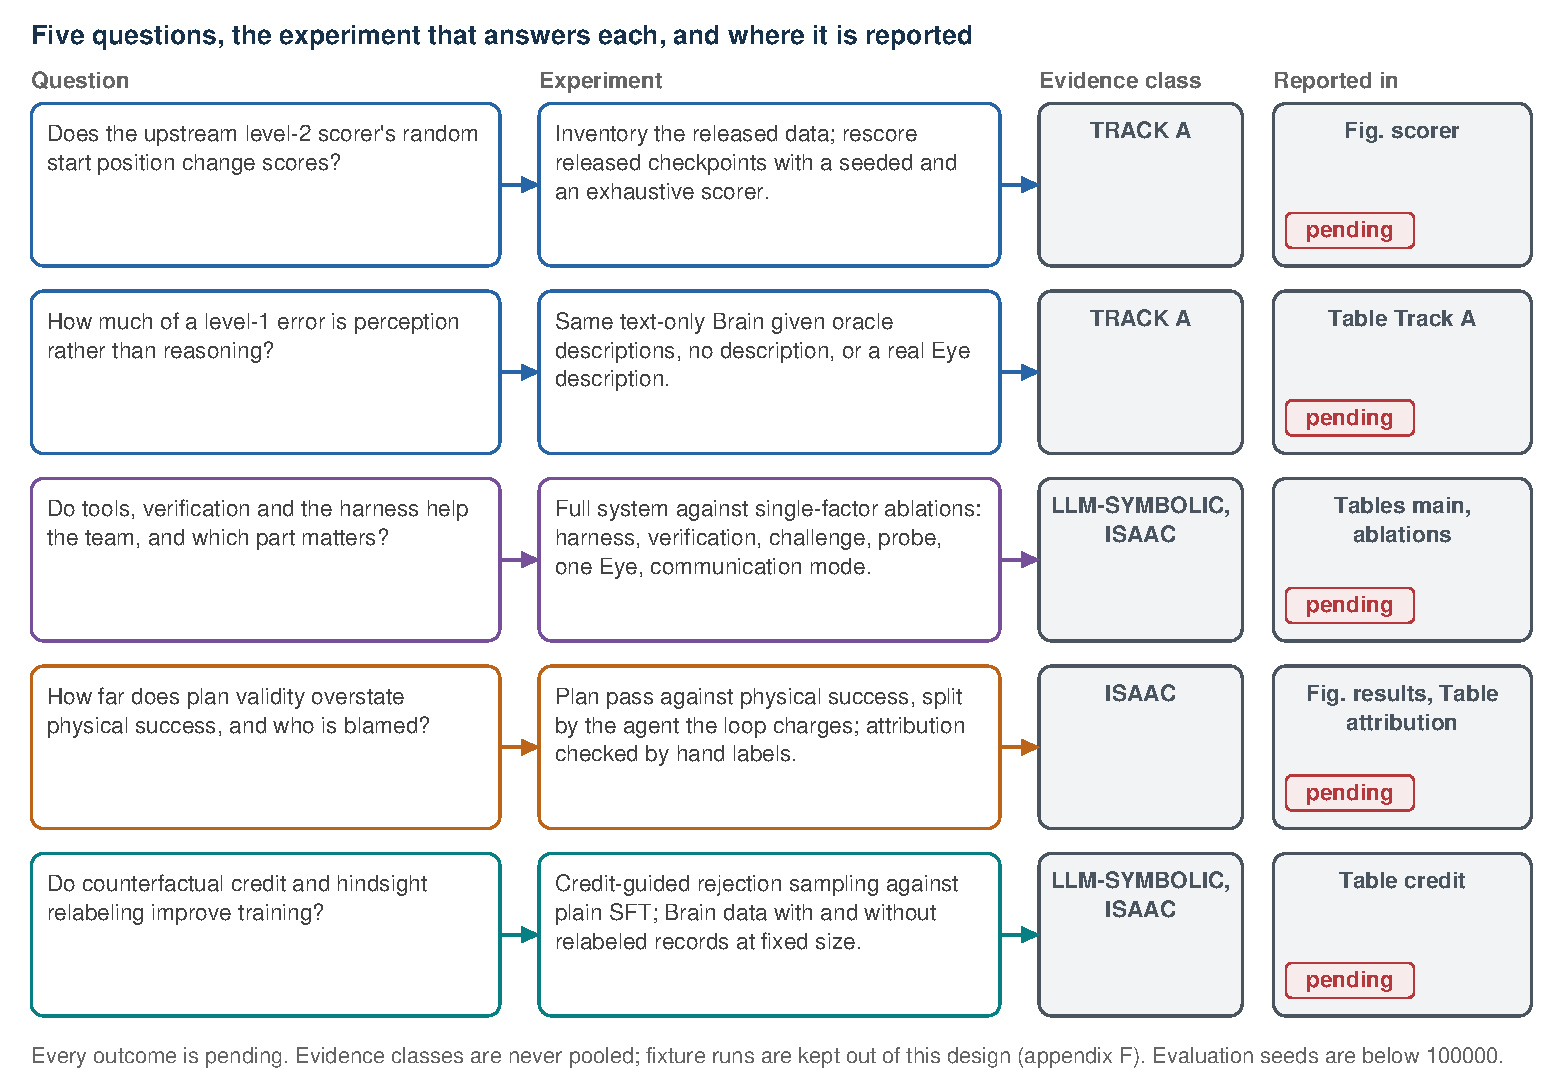
\includegraphics[width=0.95\textwidth]{fig_design}
\caption{\textbf{Planned evaluation design.} Five questions, the experiment that answers each, its evidence class and where it is reported. Track A uses real benchmark data and released models; Track B tests the packing team. Every outcome is pending, and fixture runs are kept out of the design (appendix~F).}
\label{fig:design}
\stalefig{the evidence-class column no longer matches what has actually been measured: the ISAAC class is drawn as if Isaac Lab manipulation episodes exist, whereas the only measured Newton evidence is the falling-cube rgb/depth gates G-3 (\texttt{reports/g3\_sim.json}, \texttt{reports/g3\_sim\_t4.json}), the simulation-only impedance cross-check G-6, the SIM-ABSTRACT compliance supervisor G-6b and the SIM-POSE A1 kinematics measurement. Split ISAAC into a GATE class (G-1/G-2/G-3/G-6/G-6b/A1/G-14, stating what each does and does not show) and a SIM/MODEL class (planned, not run); mark G-5, G-7, G-13, the arm runbook A1--A10 and the data-generation gates DG-1--DG-5 as not passed, mark the asset-based scene and scene bundle as not built, and keep ``every outcome is pending'' and the rule that classes are never pooled.}
\end{figure*}

\begin{table}[tbp]
\centering\small
\begin{tabular}{lp{0.3\linewidth}p{0.22\linewidth}l}
\toprule
Evidence class & What it is & Status in this version & Where reported \\
\midrule
TRACK A & Real VIKI-Bench data, real released models & \todo{pending} & \cref{tab:trackA} \\
ISAAC & Physics episodes in Isaac Lab & \todo{pending} & \cref{tab:main} \\
LLM-SYMBOLIC & A served LLM Brain on the symbolic task & \todo{pending} & \cref{tab:main,tab:ablations} \\
FIXTURE & Scripted Brain, flaky-planner wrapper, parametric Eyes & run (mechanism checks only) & \cref{app:fixture} \\
Engineering & Wiring tests on CPU with a tiny random model & run (proves wiring, not quality) & \cref{app:env} \\
\bottomrule
\end{tabular}

\caption{Evidence classes. A number is reported under exactly one class and never pooled with another.}
\label{tab:evidence}
\end{table}

\subsection{Protocol}\label{sec:protocol}
\paragraph{Evidence classes.}
TRACK~A is real VIKI-Bench data with real released models; ISAAC is physics episodes in Isaac Lab 3.0 with Newton (no Isaac Sim, no PhysX); LLM-SYMBOLIC is a served language-model Brain on the symbolic task; FIXTURE is a scripted Brain with a flaky-planner wrapper and parametric Eyes, used only to check mechanisms; engineering tests prove that code runs.
Each reported number carries its class.
\paragraph{Seeds and statistics.}
Training and data seeds are at least 100000 and evaluation seeds are below 100000, so no evaluation episode is in the training set.
Success rates are reported with Wilson 95\% intervals, and comparisons between conditions with paired bootstrap intervals over seeds; the claim a comparison supports is stated with its interval, never a bare rate.
Random draws are keyed so that conditions see the same episodes.
\paragraph{Compute.}
\todo{Compute is dual T4 GPUs on Kaggle (two 16\,GB cards), but the trainer and the G-3 scene step \emph{one device at a time}; no DDP training or two-GPU simulation exists (D-50, D-56). Confirm the memory plan for fine-tuning with fp16 LoRA without bf16, the model sizes that fit and the run times. Measured: the 4050 budget is 512 tokens for a forward/backward pass and 256 for SFT with adapters and optimizer state (D-38, D-47); the Newton-only stack passes G-3 on both the 4050 and a Kaggle T4 (D-39, D-51), where the rate is a JIT-warm-up artefact, not a throughput comparison.}

\subsection{Gates, not results}\label{sec:gates}
A gate is an engineering pass/fail criterion with a report under \texttt{reports/}; a measured gate is never pooled with a model-quality or hardware result, and a row without a report is not done.
\begin{itemize}[leftmargin=*,itemsep=1pt]
\item \textbf{Measured engineering gates.} G-1, the real Qwen3.5-4B module map (\texttt{reports/qwen35\_modules.json}); G-2, the DeltaNet fast path (\texttt{reports/g2\_fastpath.json}); G-3, Newton-only rgb/depth stepping on both the RTX~4050 and a Kaggle T4 (\texttt{reports/g3\_sim.json}, \texttt{reports/g3\_sim\_t4.json}) --- a falling cube, one device at a time, not manipulation; G-14, real-weight QLoRA SFT with a mid-epoch resume from our private repository (\texttt{reports/sft\_smoke.json}) --- a four-step smoke, not a trained model.
\item \textbf{Compliance and kinematics, by evidence class.} G-6 is a simulation-only impedance cross-check (\texttt{reports/g6\_impedance.json}); G-6b measures the compliance supervisor on a SIM-ABSTRACT point mass (\texttt{reports/g6b\_compliance.json}); step A1 measures FR3 flange forward kinematics against Newton to 0.00224\,mm over 102 configurations (\texttt{reports/g5\_reach.json}), SIM-POSE and kinematics only. None is a safety certification.
\item \textbf{Arm gates, not passed.} G-5 covers loading the FR3/FR3 Duo and Franka Hand in Newton with an effort-mode override (\texttt{reports/g5\_fr3.json}); G-7 covers external wrench injection with multiple solver substeps (\texttt{reports/g7\_wrench.json}); G-13 covers SimReady ingestion into Newton (\texttt{reports/g13\_usd\_ingest.json}, partial); the arms-first runbook A1--A10 ends in certification cards and outcome tables (\texttt{reports/arm\_cert\_*.json}, \texttt{skill\_tables/manifest.json}). \todo{No manipulation, push or arm-certification report exists; only the A1 kinematics half of G-5 is measured. Hardware/L0/L1 sign-off is assigned to a separate future track (D-22).}
\item \textbf{Data-generation gates, not passed.} DG-1--DG-5 cover the hosted Haiku run, the GPU-kernel roster, replay of real records, the first memory iteration and an image turn (design and cost estimates in the Kaggle data-generation notes). \todo{The hosted loop is built and fixture-tested on SIM-POSE; no Kaggle endpoint has been called and no frontier model has run.}
\end{itemize}

\subsection{Held-out benchmark matrix}\label{sec:matrix}
The held-out test set uses seeds below 100000 exclusively, with at least 30 episodes per family: packing variants, heavy/fragile ordering, occlusion-heavy arrangements, distractors, handover-required cases, human-push interruption, kitchen tasks on SimReady objects, and unseen layouts and objects.
The matrix is exact (D-64): M1, base Qwen3.5-4B zero-shot; M2, base Qwen3.5-9B zero-shot; M3, 4B SFT; M4, 4B SFT with GRPO at $k=4$; M5, 4B SFT with GRPO at $k=8$; M6, frontier models zero-shot; M7, the same frontier models in the harness (skills, tools, memory, rules and success/failure-memory retrieval); M8, base 4B in the harness.
The isolated effects are SFT (M3 minus M1), GRPO at $k=4$ and $k=8$ (M4 and M5 minus M3), the harness on frontier models (M7 minus M6) and on the base 4B (M8 minus M1).
Metrics include success, plan pass, per-family success, localisation, occlusion handling, eye-tool use, two-arm coordination, recovery, collisions and compliance (push deflection, settle time, return speed and plan-pause correctness), each with Wilson intervals and paired bootstrap over seeds; every cell traces to a run card carrying a config hash, seed list and model revision.
\todo{This matrix is a protocol only: no row has a measured number, and the frontier rows in eval mode have not been run.}

\subsection{Track A: real benchmark data and released models}\label{sec:track-a}
Track A re-evaluates the released VIKI-R checkpoints on VIKI-Bench with our own runner, and decomposes a level-1 error into perception and reasoning by giving a text-only Brain oracle descriptions, no description, or a real Eye description of the same image (\cref{tab:trackA}).
If compute allows, a matched-base control trains the same base model with the upstream recipe, so that any difference from our additions is attributable.
\todo{Pin the upstream VIKI-R repository commit and dataset revision; record licences.}

\begin{table}[tbp]
\centering\small
\begin{tabular}{p{0.40\linewidth}cccc}
\toprule
Condition & L1 accuracy & L2 accuracy & Format rate & Failed items \\
\midrule
Released VIKI-R checkpoints, upstream-style scoring & \todo{pending} & \todo{pending} & \todo{pending} & \todo{pending} \\
Released checkpoints, position-robust scoring, full split & \todo{pending} & \todo{pending} & \todo{pending} & \todo{pending} \\
Text-only Brain with oracle descriptions & \todo{pending} & \todo{pending} & \todo{pending} & \todo{pending} \\
Same Brain, no Eye description & \todo{pending} & \todo{pending} & \todo{pending} & \todo{pending} \\
Same Brain, real Eye description & \todo{pending} & \todo{pending} & \todo{pending} & \todo{pending} \\
Matched-base control (Qwen2.5-VL-3B), if compute allows & \todo{pending} & \todo{pending} & \todo{pending} & \todo{pending} \\
\bottomrule
\end{tabular}

\caption{Track A design. L1 and L2 are VIKI-Bench levels. All cells are pending.}
\label{tab:trackA}
\end{table}

\subsection{An audit of the upstream level-2 scorer}\label{sec:scorer}
We read the upstream level-2 scoring code.
It checks a plan with a pure-Python feasibility function, so no simulator is involved; for each asset it draws a start position with \texttt{random.choice} on every call, and a plan counts as correct if it is feasible and the ratio of reference length to plan length is at least 0.99; the reward is 0.1 for format plus 0.9 for correctness.
The evaluation scripts read only the first 900 level-2 rows and the first 1000 level-1 rows, and the level-2 script loads one split file but writes to a directory with another name.
\Cref{fig:scorer} shows the consequence on a toy case we built: if a plan is valid only for some start positions, an unseeded scorer passes it by luck of the draw.
In the toy case, 40 unseeded draws pass 18 times, the exhaustive average over start positions is 0.5, and a position-agnostic plan passes 40 of 40.
This is a synthetic demonstration of the mechanism; how many real VIKI-Bench items depend on a random start position is unknown until the inventory script runs on the dataset, and we make no claim about the published numbers.
\todo{Run the inventory on the released data; report the fraction of items affected, and rescore the released checkpoints with a seeded and an exhaustive scorer.}

\begin{figure*}[tbp]
\centering
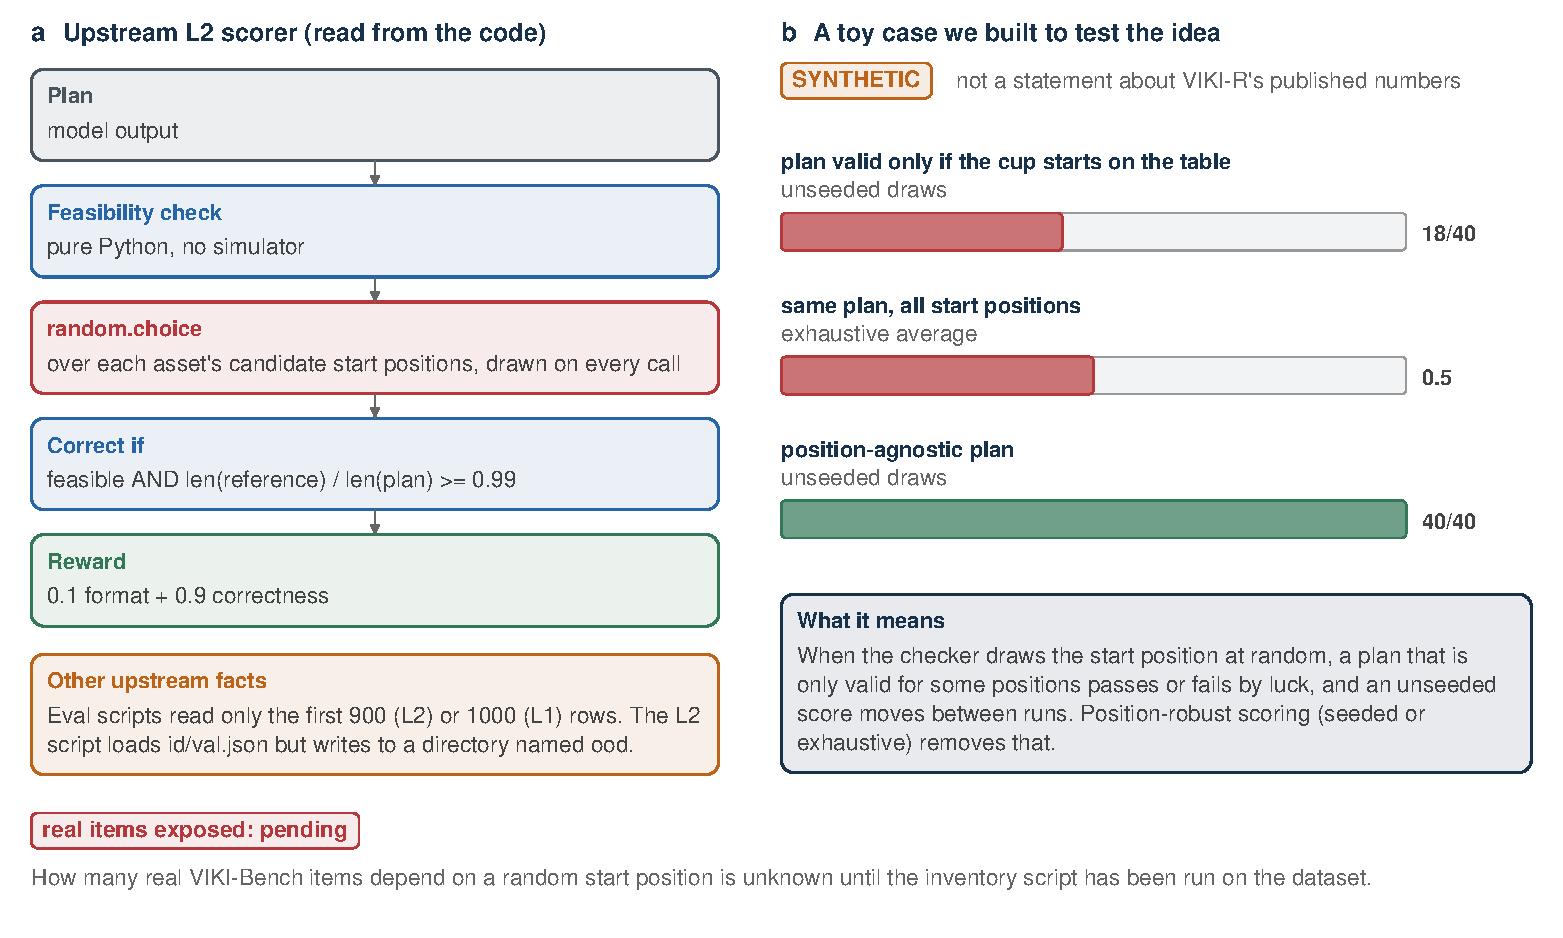
\includegraphics[width=\textwidth]{fig_scorer_audit}
\caption{\textbf{Audit of the upstream level-2 scorer.} (a)~The scoring path as read from the code; the highlighted step draws start positions at random on every call. (b)~A synthetic toy case: a plan valid only for some start positions passes 18 of 40 unseeded draws, has an exhaustive average of 0.5, and a position-agnostic plan passes 40 of 40. The toy case is not a statement about the published VIKI-R numbers.}
\label{fig:scorer}
\end{figure*}

\subsection{Track B: the packing team}\label{sec:track-b}
Track B runs the team on procedurally generated packing tasks, in the symbolic world with a served Brain (LLM-SYMBOLIC) and in Isaac Lab (ISAAC) (\cref{tab:main}).
The headline measurement is the gap between plan validity and physical success: the fraction of episodes whose plan passes the dry run but whose physical episode fails, split by the agent the loop charges.
\Cref{fig:results} draws the results from the results bundle when one exists, and is otherwise a red placeholder.

\begin{table}[tbp]
\centering\small
\begin{tabular}{p{0.36\linewidth}cccc}
\toprule
Condition (Track B, one evidence class per run) & Success [95\% Wilson] & Plan pass & Replans & Msg tokens \\
\midrule
Full system, LLM-SYMBOLIC & \todo{pending} & \todo{pending} & \todo{pending} & \todo{pending} \\
Full system, ISAAC & \todo{pending} & \todo{pending} & \todo{pending} & \todo{pending} \\
\bottomrule
\end{tabular}

\caption{Track B main results (pending). Success with a Wilson interval, the fraction of plans passing the dry run, replans per episode and message tokens.}
\label{tab:main}
\end{table}

\begin{figure*}[tbp]
\centering
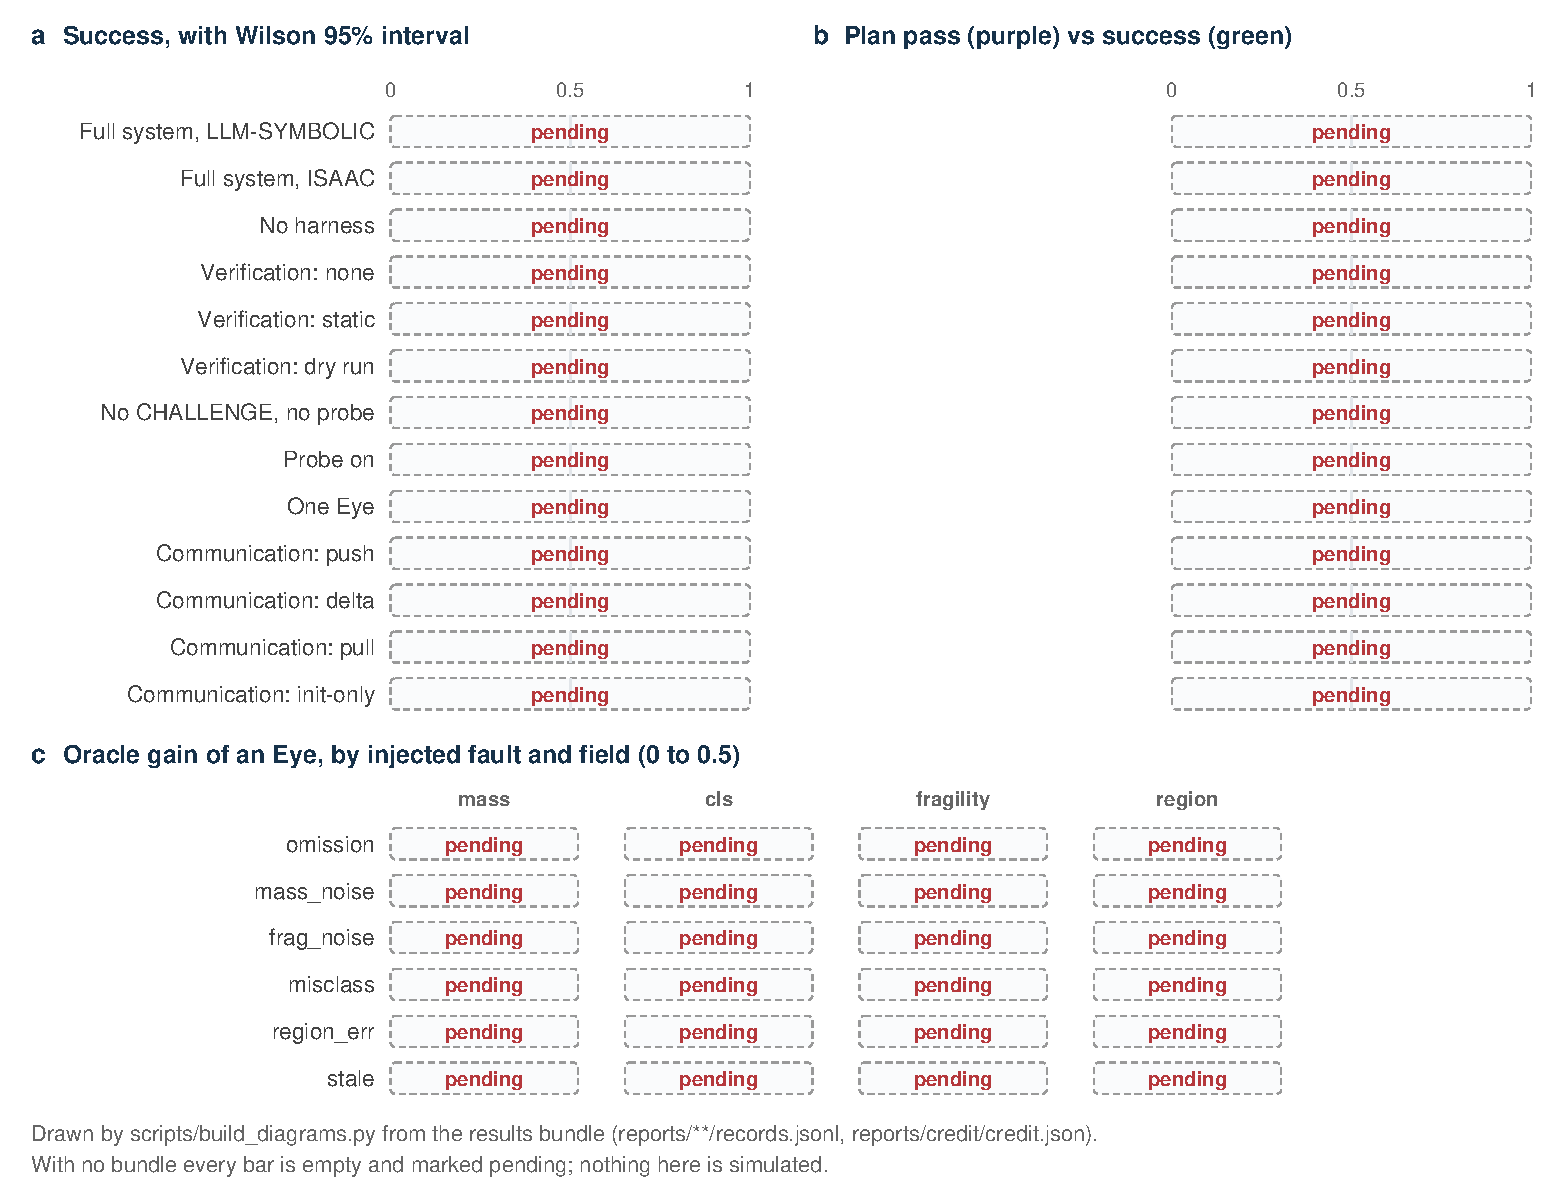
\includegraphics[width=0.95\textwidth]{fig_results}
\caption{\textbf{Results figure, generated from the results bundle.} (a)~Success per configuration with Wilson intervals. (b)~Plan pass against success. (c)~Oracle gain by injected fault and field. With no bundle present every bar is empty and marked pending; nothing here is simulated.}
\label{fig:results}
\end{figure*}

\subsection{Ablations}\label{sec:ablations}
\Cref{tab:ablations} lists the ablations: the harness, the three verification modes, challenge and probe, one Eye against two, and the four communication modes.
Each is a code configuration, so the comparison differs in one factor.
\begin{table}[tbp]
\centering\small
\begin{tabular}{p{0.36\linewidth}cccc}
\toprule
Ablation & Success [95\% Wilson] & Plan pass & Replans & Msg tokens \\
\midrule
No harness & \todo{pending} & \todo{pending} & \todo{pending} & \todo{pending} \\
Verification: none & \todo{pending} & \todo{pending} & \todo{pending} & \todo{pending} \\
Verification: static & \todo{pending} & \todo{pending} & \todo{pending} & \todo{pending} \\
Verification: dry run & \todo{pending} & \todo{pending} & \todo{pending} & \todo{pending} \\
No CHALLENGE, no probe & \todo{pending} & \todo{pending} & \todo{pending} & \todo{pending} \\
Probe on & \todo{pending} & \todo{pending} & \todo{pending} & \todo{pending} \\
One Eye & \todo{pending} & \todo{pending} & \todo{pending} & \todo{pending} \\
Communication: push & \todo{pending} & \todo{pending} & \todo{pending} & \todo{pending} \\
Communication: delta & \todo{pending} & \todo{pending} & \todo{pending} & \todo{pending} \\
Communication: pull & \todo{pending} & \todo{pending} & \todo{pending} & \todo{pending} \\
Communication: init-only & \todo{pending} & \todo{pending} & \todo{pending} & \todo{pending} \\
\bottomrule
\end{tabular}

\caption{Ablations (pending).}
\label{tab:ablations}
\end{table}

\subsection{Counterfactual credit and hindsight}\label{sec:credit-eval}
We evaluate the credit signal on whether rejection sampling guided by it produces Eyes with a smaller oracle gain than plain fine-tuning, and report the gain with its field breakdown (\cref{tab:credit}).
The fixture version of the credit estimate, which checks that the estimator recovers the injected fault, is in appendix~F.
For hindsight relabeling we compare Brain training with and without relabeled records at fixed total size.
\begin{table}[tbp]
\centering\small
\begin{tabular}{p{0.28\linewidth}ccccc}
\toprule
Eye variant & Oracle gain G & mass & class & fragility & region \\
\midrule
Plain SFT Eye & \todo{pending} & \todo{pending} & \todo{pending} & \todo{pending} & \todo{pending} \\
Rejection-sampled Eye & \todo{pending} & \todo{pending} & \todo{pending} & \todo{pending} & \todo{pending} \\
Fixed-Brain counterfactual & \todo{pending} & \todo{pending} & \todo{pending} & \todo{pending} & \todo{pending} \\
\bottomrule
\end{tabular}

\caption{Oracle gain $G$ of trained Eyes and its breakdown by field (pending).}
\label{tab:credit}
\end{table}

\subsection{Is the attribution right?}\label{sec:attribution-eval}
The attribution rules are heuristics, so we check them against hand labels on a sample of failed episodes and report agreement and Cohen's $\kappa$ per agent (\cref{tab:attribution}).
\todo{Choose the number of episodes to hand-label and who labels them.}
\begin{table}[tbp]
\centering\small
\begin{tabular}{lccc}
\toprule
Agent label & Episodes labelled by hand & Agreement with the heuristic & Cohen's kappa \\
\midrule
Eye & \todo{pending} & \todo{pending} & \todo{pending} \\
Brain & \todo{pending} & \todo{pending} & \todo{pending} \\
Arm & \todo{pending} & \todo{pending} & \todo{pending} \\
\bottomrule
\end{tabular}

\caption{Agreement of the loop's attribution with hand labels (pending).}
\label{tab:attribution}
\end{table}
